\documentclass[10pt, a4paper]{article}

\usepackage{graphicx} 
\usepackage{natbib}
\bibpunct{(}{)}{;}{a}{}{,}  % to adjust punctuation in references
\usepackage[utf8]{inputenc}
\usepackage[margin=10pt, font=small, labelfont=bf]{caption} 
\usepackage[margin=1in]{geometry}
\usepackage{color}
\usepackage{xcolor}
\usepackage[]{hyperref}
\definecolor{darkblue}{rgb}{0,0,.5}
\hypersetup{colorlinks=true, breaklinks=true, linkcolor=darkblue, menucolor=darkblue, urlcolor=darkblue, citecolor=darkblue}
\usepackage{multicol}              
\usepackage{multirow}
\usepackage{booktabs}  
\usepackage{enumerate}
\usepackage{subcaption}
\usepackage{eurosym}
\usepackage{color}
\usepackage{siunitx}
\usepackage{lineno} % for line numbers 
\usepackage{setspace}
%\usepackage{float}
\usepackage{listings}
\usepackage{xfrac}
\usepackage[T1]{fontenc}
%\usepackage{pygmentize}
%\usepackage{minted}

\definecolor{middlegray}{rgb}{0.5,0.5,0.5}
\definecolor{lightgray}{rgb}{0.8,0.8,0.8}%
\definecolor{orange}{rgb}{0.8,0.3,0.3}
\definecolor{yac}{rgb}{0.6,0.6,0.1}

\lstset{
	basicstyle=\small\ttfamily,
	keywordstyle=\bfseries\ttfamily\color{orange},
	stringstyle=\color{blue}\ttfamily,
	commentstyle=\color{teal}\ttfamily,
	emph={square}, 
	emphstyle=\color{blue}\texttt,
	emph={[2]root,base},
	emphstyle={[2]\color{yac}\texttt},
	flexiblecolumns=false,
	tabsize=2,
	xleftmargin=5pt
}

% Default fixed font does not support bold face
%\DeclareFixedFont{\ttb}{T1}{txtt}{bx}{n}{10} % for bold
%\DeclareFixedFont{\ttm}{T1}{txtt}{m}{n}{10}  % for normal

% Custom colors
%\usepackage{color}
%\definecolor{deepblue}{rgb}{0,0,0.5}
%\definecolor{deepred}{rgb}{0.6,0,0}
%\definecolor{deepgreen}{rgb}{0,0.5,0}
% Python style for highlighting
%\newcommand\pythonstyle{\lstset{
%	language=Python,
%		basicstyle=\ttm,
%		otherkeywords={self},             % Add keywords here
%		keywordstyle=\ttb\color{deepblue},
%		emph={MyClass,__init__},          % Custom highlighting
%		emphstyle=\ttb\color{deepred},    % Custom highlighting style
%		stringstyle=\color{deepgreen},
%		frame=tb,                         % Any extra options here
%		showstringspaces=false            % 
%}}

\setlength\parindent{0pt}
% Python environment
\lstnewenvironment{python}[1][]
{
	\pythonstyle
	\lstset{#1}
}
{}


\begin{document}
	
	\markboth{}
	\\\noindent University of Freiburg \hspace{10cm}  July 6, 2018
	\\Faculty of Environment and Natural Resources
	\\Module: GIS Plus
	\\Lecturer: João Paulo Pereira
	\\Module Coordinator: Holger Weinacker
	\\Authors: Luka Kern, Nele Stackelberg and Felix Rentschler
	\\
	
	\begin{center}
		\huge{Project 06: Rasterizer Function} \vspace{0.5cm}\\
		%\Large {Rasterizer}
	\end{center}
	
	%\maketitle
	\
	\onehalfspacing % larger vertical space between lines 
	%\linenumbers
	%\tableofcontents
	
	
	\section{Aim of the Project}
	The aim of this project was to create a rasterizing tool in \texttt{Python}, that generates a raster file from a given shapefile. The idea of such a rasterizing tool is to load the geometries of a shapefile into a geometry collection, implement a regular grid within the bounding box of this geometry collection and assign a value to each grid cell. For the value assignment it is either possible to use attribute values of the geometry or to use a binary format depending on the presence of a geometry.
	
	\subsection*{Approach}\label{doc}
	To achieve this task first of all we developed a script which randomly generates geometries -- polygon, point and line -- and saves them as shapefiles. Those shapefiles can serve as test data. The rasterizing tool is implemented as a function with several options for the user, whereby the filepath to a shapefile is the essential argument. The function works according to the following pattern: The geometries of the given shapefile are loaded into a geometry collection. Then the bounding box around this collection is defined with an additional frame. Within this frame a regular grid is generated, as well as point geometries representing each grid cell. With the coordinates of the generated point geometries it is possible to run geometric queries, testing if a positive value should be assigned to the pixel. Regarding the value assignment, the function is using a binary format with a highlighting of ovelapping geometries. Finally the raster can be saved in a \SI{8}{Bit} format as a TIFF file.
	
	\section{Structure of the Function}
	The path of the shapefile is the function's first argument. 
	The second argument is the amount of pixel, which is used as a proxy for the resolution. The buffersize and the name of the output file can additionally be defined as arguments for the function. Furthermore, the user has the opportunity to specify the name of the resulting file, to preview the result inline, as well as suppressing the saving of the TIFF file.
	For the case, that no shapefile is available to run the function, the user can generate random geometries with the provided script (see section  \ref{doc}).
	
	\subsection*{Import the Shapefile}
	To open the shapefile, the \texttt{fiona} package is used. Every geometry object of the shapefile is stored in a geometry collection from the \texttt{shapely.geometry} package.
	
	\subsection*{Calculate the Resolution}
	To calculate the resolution, the minimum and maximum dimension of the geometry collection on the x- and y- axes are extracted.  Those values are used to determine the range dimension. 
	
	The resolution depends on the amount of pixel in each dimension. To determine the resolution, the mean range dimension is divided by the amount of pixel, given as input of the function. The mean of x- and y-range is used in this calculation, because the two values may differ. 
	
	\subsection*{Define the Bounding Box and create the Grid}
	 A minimum bounding box is defined as the maximum spatial extension of the geometry collection. Additionally, the buffer value creates a visual frame around the minimum bounding box. The purpose of this step is to present the objects with distance to the margin in the resulting image. Therefore the argument ``buffer'' describes the amount of pixel in the bounding box.  To transform the pixel value to the coordinates, it is multiplied with the resolution, resulting in the width of the bounding box. The dimension of the geometry collection (xmin, ymin, xmax, ymax) is used to define the dimension of the outer frame of the bounding box by adding and subtracting its width.
	
	The outer frame's minimum and maximum coordinate values (dimension) of the bounding box are used to create a grid with the function \textit{mgrid} from the \texttt{numpy} package. The coordinates of every grid cell (pixel) are saved as point geometries. Those geometries are stored in a list.
	%bis geom_pixel beschreiben
	
	\subsection*{Within Query}\label{within}
	The information about every grid cell's coordinates allows a geometric query, which depends on the geometry type. 
	In case it is a point, the query checks if the pixel's position  equals the point's position ($\pm 0.5*resolution$ in both x- and y-dimension) in the vector data. The addition, respectively subtraction of 0.5 times the resolution ensures that every point is detected, even if it is not the center of the grid cell. 
	If the vector geometry is a line, a buffer around the line is calculated. The \textit{within}-function of the \texttt{shapely} package is used to query if a point is in this buffer. A similar query is also used for polygon geometries, whereby the \textit{within} function is applied directly to the polygon and not to a buffer.
	The query is applied to all geometries of the geometry collection. The result for each geometry is a list with boolean values. These lists are appended stepwise as sublists to an empyt list.
	
	\subsection*{Create an Array}
	In the next step the sublists are combined to assign a value to each pixel. Therefore the sum off all sublist is written to a new list, whereby the sum of boolean values is the amount of ``True'' values.  Afterwards an array with the size of the grid is created by transforming the list into sublists. The length of each sublist is determined by the number of pixel on the x-axis. The resulting format can be transformed to a \texttt{numpy} array.
	
	\subsection*{Set Radiometric Resolution}
	To ensure all values of the array will be displayed in the \SI{8}{Bit} TIFF file, the values are rescaled between 0 and 255. The calculation of each value $x_{i\_new}$ from its former value $x_i$ and maximum value $x_{max}$ in the grid $x$ is computed according to the following formula:
	$ x_{i\_new} = 255 * \frac{x_i}{x_{max}} $.
	
	\subsection*{Flip Array and Save as TIFF}
	If the array was plotted at this stage, python's characteristics to show the y-axis the reverse way, would result in an inverted image. Therefore the array is flipped upside down with the \textit{flipud} function of the package \texttt{numpy}.
	After all this has been computed, the result can be saved as TIFF file. For this purpose the \texttt{scikit} package provides the \textit{imsave} function, which is used here.
	
	\section{Result}
	Examples of the function's output are shown below, side by side to their origin shapefiles. For each geometry type, there is one figure. Figure \ref{fig:line} and \ref{fig:poly} show the rasterized images of randomly generated test shapefiles. For the point geometry (figure \ref{fig:points}) a shapefile was used that shows 606 points indicating the location of various cities.   
	
	\hfill
	%-------- LINE --------%
	\begin{figure}[htbp]
		\centering
		\begin{subfigure}{.5\textwidth}
			\centering
			
\includegraphics[width=5cm]{images/lines_vector.png}
			\caption{Vector}
		\end{subfigure}%
		\begin{subfigure}{.5\textwidth}
			\centering
			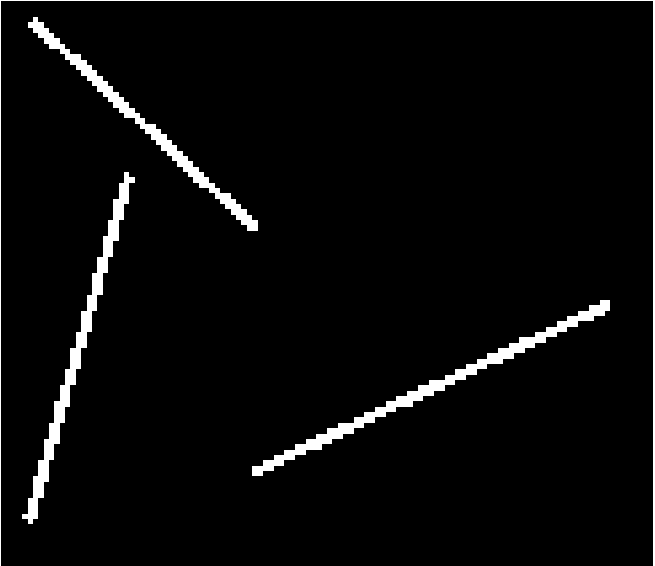
\includegraphics[ width=5cm]{images/lines_raster.png}
			\caption{Raster}
		\end{subfigure}
		\caption{Line type geometry: the original vector data file on the left (a) as well as the converted raster file on the right (b). The function's arguments to create the raster file: pixel=100, buffer=10 }
		\label{fig:line}
	\end{figure}
	\hfill
	
	%-------- POLYGON --------%
	\begin{figure}[htbp]
		\centering
		\begin{subfigure}{.3\textwidth}
			\centering
			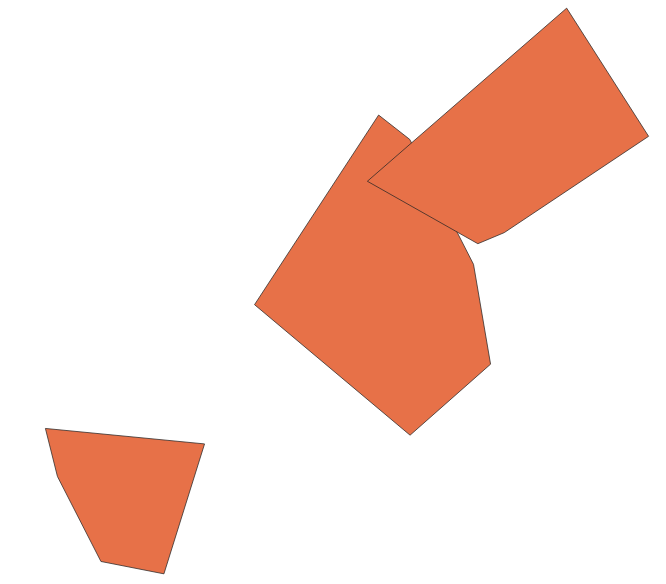
\includegraphics[ width=4cm]{images/polys_vector.png}
			\caption{Vector}
		\end{subfigure}%
		\begin{subfigure}{.3\textwidth}
			\centering
			
\includegraphics[ width=4cm]{images/polys_raster_low_res.png}
			\caption{Raster low resolution}
		\end{subfigure}
		\begin{subfigure}{.3\textwidth}
			\centering
			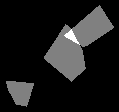
\includegraphics[ width=4cm]{images/polys_raster_high_res.png}
			\caption{Raster high resolution}
		\end{subfigure}
		\caption{Polygon type geometry rasterized with different resolution: the original vector data file on the left (a) as well as the converted raster file on the right (b, c). The function's arguments to create the raster file b: pixel=20, buffer=5 and raster file c: pixel=100, buffer=10}
		\label{fig:poly}
	\end{figure}
	%lines, poly high: 100, 10
	% cities: 100, 5
	% poly low: 20, 5
	
		%-------- POINTS --------%
	\begin{figure}[htbp]
		\centering
		\begin{subfigure}{.5\textwidth}
			\centering
			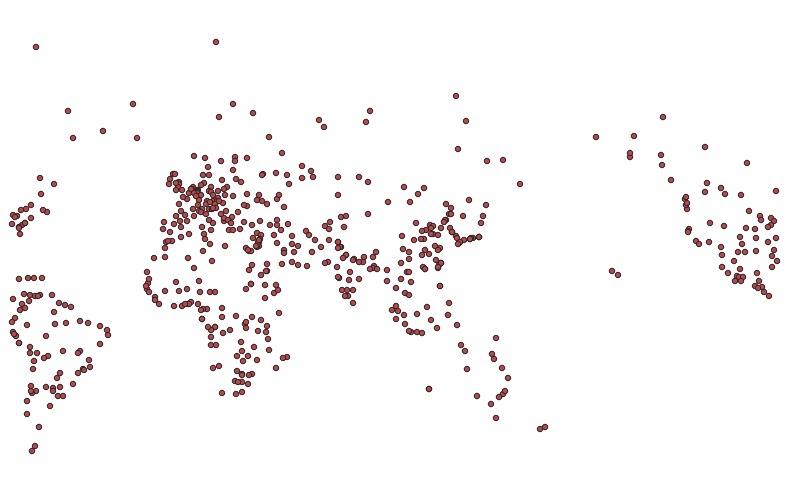
\includegraphics[ width=6.5cm]{images/points_vector.png}
			\caption{Vector}
		\end{subfigure}%
		\begin{subfigure}{.5\textwidth}
			\centering
			
\includegraphics[ width=7.5cm]{images/points_raster.png}
			\caption{Raster}
		\end{subfigure}
		\caption{Point type geometry: the original vector data file on the left (a) as well as the converted raster file on the right (b). The function's arguments to create the raster file: pixel=100, buffer=5}
		\label{fig:points}
	\end{figure}
	\newpage
%	\hfill
	\section{Issues}
	
	\subsection*{Solved Issues}
	To provide a general function, that can be applied to a shapefile, no matter if the geometry type was point, line or polygon, those three possibilities had to be covered. The solution of this issue should have become clear in the section \ref{within} (Within query).\
	
	To set the function's argument ``resolution'' instead of the ``pixel'' would have been a more intuitive value. We did not use this argument because of the following reason:
	The runtime of the function mainly depends on the raster file's resolution. To set an appropriate resolution, the user has to know the range of coordinate values (and the reference system) in the shapefile and divide it by the amount of pixel. For raster images with increasing pixel in one dimension, the runtime increases exponentially.  During development the function was applied to shapefiles, of which dimensions and reference system were unknown, therefore the approximate amount of pixel seemed to be the more convenient argument.\
	
	To make the group work as efficient as possible, especially since not all participants were able to be in Freiburg, the platform GitHub was chosen to facilitate the workflow. The repository \url{https://github.com/lukakern/GisPlus.git} was created for the project. Since working with git as version-control in the console or using the software pyCharm was new to all group members, there were some difficulties in handling the files by merging, pushing and pulling. It took time until these issues were solved, but it was worth it, especially since these experiences will be very helpful for future projects.
	
	\subsection*{Issues in Progress}
	As a result the function creates raster files where the presence or absence of the shapefile geometries is displayed and overlapping geometries are represented by lighter gray values. This is a possibility that works for all given shapefiles. However the representation of attributes in the raster file by different gray values or even raster bands would ensure a broader application of the function.\
	
	Different users may also want to be able to choose from different radiometric resolutions for the output TIFF file instead of the hard-coded \SI{8}{Bit} resolution in the function. Therefore it would be nice to have the resolution as an argument for the function.\
	
	The function saves the TIFF file without reference system. This is probably a problem for many users, as the image cannot easily be used for further processing in standard GIS-software. To include this feature to the function the reference system (EPSG number) of the input shapefile has to be accessed in the beginning of the function and reused when writing the TIFF file.
	
	\begin{figure}[!htbp]
		\centering
		%	\includegraphics[width=16cm]{wildfire.png}
		%	\caption{Wildfire event in a boreal forest}
	\end{figure}
	
	
	
	
\end{document}